\documentclass{article}

\title{BertonGan: a conditional GAN for performing various tasks}
\author{ Aaron Schindler, Herbert Wright }
\date{\today}

\begin{document}

% the title page
\maketitle
\pagebreak

% the introduction/background section
\section{Introduction}

\subsection{Generative Adversarial Networks}

Generative Adversarial Networks were introduced by Ian Goodfellow \cite{goodfellow2020generative}.

% the methods section
\section{Methods}

\subsection{BertonGan structure}

Our approach is to train an encoder-decoder while also simultaneously training the discriminator network. Both the decoder and discriminator(s) will be conditioned on a latent variable that provides all necessary facial information. The discriminator(s) will give two values corresponding to whether or not the reconstructed image is fake and if the image also corresponds to the latent variable it has been conditioned on. The four network components of our project are outlined below: \\
\begin{enumerate}
\item Face encoder network: $f_F: \mathbb{R}^{n\times W \times H} \rightarrow \mathbb{R}^{h_f}$
\begin{enumerate}
\item Input: $n$ images of the same subjects face
\item Output: A latent representation of the subjects face
\end{enumerate}
\item Image encoder network: $f_I: \mathbb{R}^{W \times H} \rightarrow \mathbb{R}^{h_I}$
\begin{enumerate}
    \item Input: An image of a subjects face
    \item Output: A latent representation of the image
\end{enumerate}
\item Image decoder network: $f_G: \mathbb{R}^{h_F + h_I} \rightarrow \mathbb{R}^{W \times H}$
\begin{enumerate}
    \item Input: Latent representations of a face and image
    \item Output: A reconstructed image decoded from the latent features
\end{enumerate}
\item Discriminator network: $f_D: \mathbb{R}^{W \times H} \times \mathbb{R}^{h_F} \rightarrow [0,1]^2$
\begin{enumerate}
    \item Input: An image and a latent representation of a face
    \item Output: Two probabilities
    \begin{enumerate}
        \item Probability of being a fake image
        \item Probability of being a different person than the faces encoded into the latent vector
    \end{enumerate}
\end{enumerate}
\end{enumerate}
A visual encoding of the networks described above is given below:
\begin{figure}
    \centering
    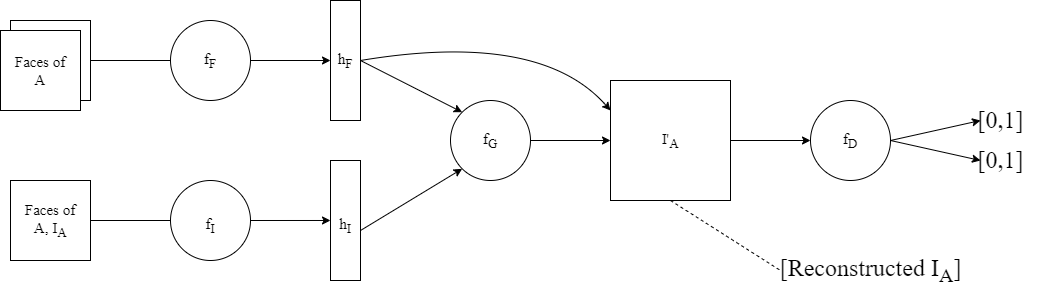
\includegraphics[scale=0.25]{OurNetwork.png}
    \caption{Figure 1 is a visual representation of our total network, comprising each of the four components above}
    \label{fig:my_label}
\end{figure}

\subsection{Networks}

\subsection{Training Procedure}


% the experiments section
\section{Experiments}

\subsection{MNIST Experiments}

\subsection{CelebA Experiments}

% the conclusion/future work section
\section{Conclusion}

\pagebreak
% \section*{References}

\bibliography{sources}
\bibliographystyle{ieeetr}

\end{document}
